\documentclass[8pt]{beamer}
\usepackage[T2A]{fontenc}                
\usepackage[utf8]{inputenc}  
\usepackage[english, russian]{babel}
\usepackage{indentfirst}
\usepackage{graphicx}
\documentclass{beamer}

\usetheme{Arguelles}
 



\title{Практикум на ЭВМ.\\ "Мечи залива работорговцев" - отчет}
\author{Фостенко О.А., Бузин Н.И., Лопухов С.А.\\ 311 группа}
\institute{МГУ имени М.В. Ломоносова, Москва, Россия}
\date{2024, 23 апреля}
 
\begin{document}
 
\frame{\titlepage}
 
\begin{frame}
\frametitle{Постановка задачи}
Для ведения войны с Семью Королевствами требуется оружие, для изготовления которого нужна сталь. Основными поставщиками стали являются две компании : {Westeros Inc.} и {Harpy \& Co}. На данный момент, товар закупается у обеих компаний, но каждая из них предлагает достаточно большую скидку, если контракт на поставку сырья будет заключен эксклюзивно с ней.\\

\bigskip
Задача: проанализировать перспективы заключения контрактов с обеими компаниями и выбрать ту, сотрудничество с которой наиболее выгодно.
\\
\end{frame}
 

\begin{frame}
\frametitle{Анализ\\{\smallРазница в производстве мечей между компаниями}}
\begin{figure}[h]
		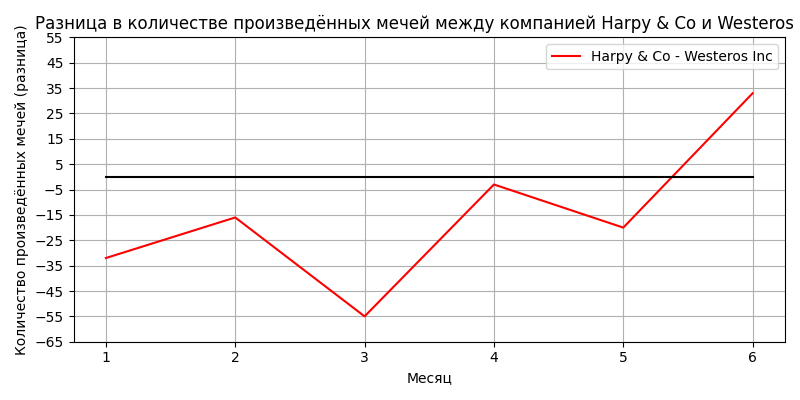
\includegraphics[width=110mm]{6-before-last.png}
		\caption{1}
		\label{First}
\end{figure}
\end{frame}

\begin{frame}
Выводы из рис.1:\\

\bigskip

Т.к. компании производят несколько тысяч единиц оружия каждый месяц (см. рис. 3), можно сказать, что разрыв по показателю "производство в месяц" незначительный\\ 

\bigskip
\\
\end{frame}

\begin{frame}
\frametitle{Анализ\\{\small Аккумулированное число дефектов, по месяцам}}
\begin{figure}[h]
		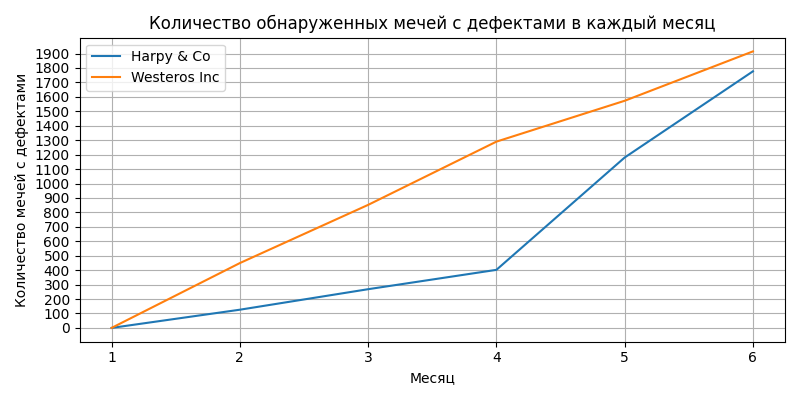
\includegraphics[width=110mm]{4-before-last.png}
		\caption{2}
		\label{Second}
\end{figure}
\end{frame}
\begin{frame}
Из рис.2 четко видно, что у компании "Westeros.inc" больше дефектов с месяцами, но у компании "Harpy.co" ближе к концу периода число дефектов растет быстрее, чем у конкурента
\end{frame}

\begin{frame}
\frametitle{Анализ\\ {\small Всего мечей произведено}}
\begin{figure}[h]
		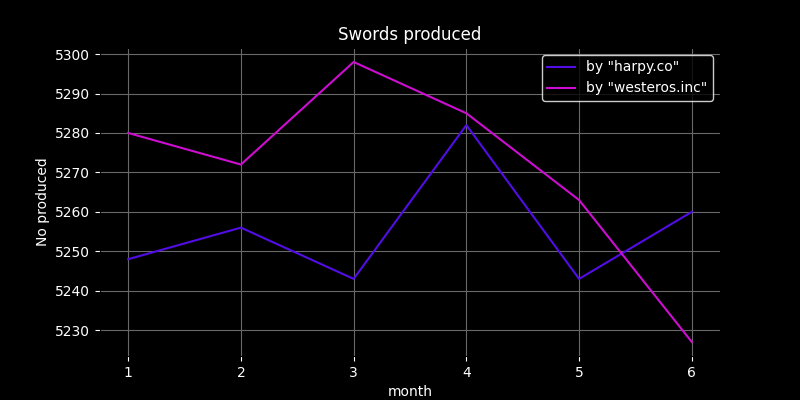
\includegraphics[width=110mm]{3-before-last.png}
		\caption{3}
		\label{Third}
\end{figure}
\end{frame}

\begin{frame}
\frametitle{Анализ\\ {\small Число дефектов (другой тип графика)}}
\begin{figure}[h]
		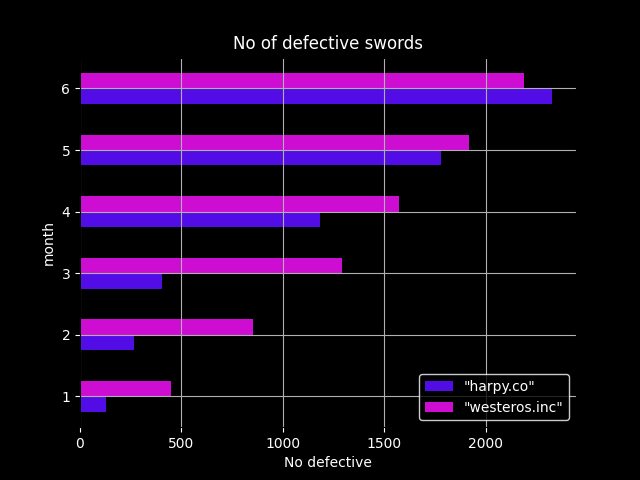
\includegraphics[width=90mm]{2-before-last.png}
		\caption{4}
		\label{Fourth}
\end{figure}
\end{frame}

\begin{frame}
\frametitle{Анализ\\ {\small}}
Видно, что в конце 6-го месяца как число дефектов, так и общее производство отличаются незначительно\\

\bigskip
\end{frame}


\begin{frame}
\frametitle{Анализ\\{\small Доля мечей, являющихся дефектными, в зависимости от компании, по месяцам}}
\begin{figure}[h]
		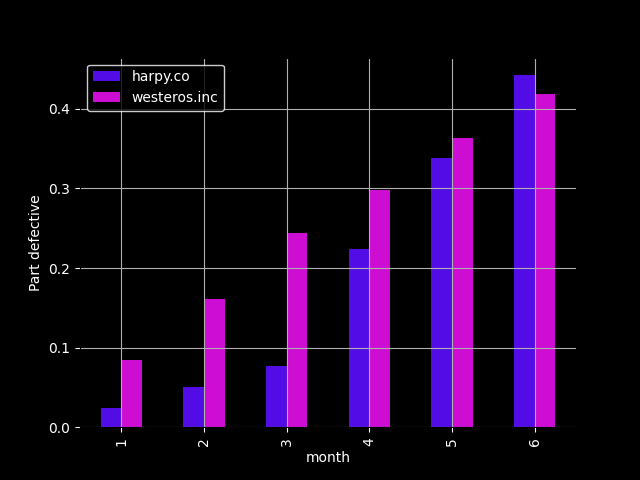
\includegraphics[width=90mm]{prelast.png}
		\caption{5}
		\label{Fifth}
\end{figure}
\end{frame}

\begin{frame}
Опять видим, что, хотя изначально Harpy.co производила более качественную сталь, число дефектных мечей к концу начало увеличиваться\\

\bigskip

\end{frame}

\begin{frame}
\frametitle{Анализ\\{\small Доля мечей, являющихся дефектными, в зависимости от компании, по месяцам использования (изаншивания) мечей}}
\begin{figure}[h]
		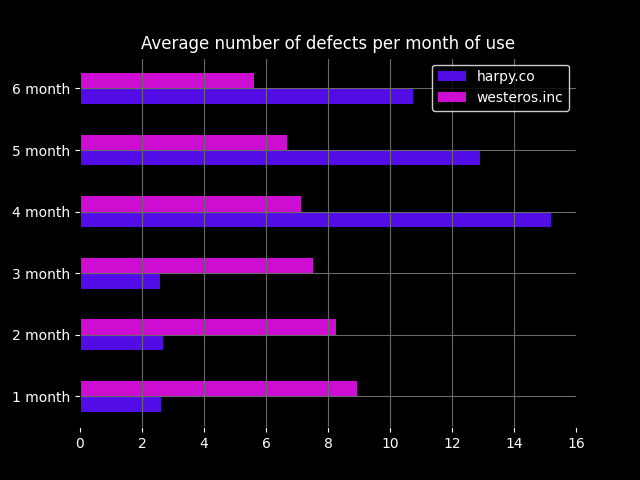
\includegraphics[width=90mm]{last.png}
		\caption{6}
		\label{Sixth}
\end{figure}
\end{frame}

\begin{frame}
А вот этот график показывает значительный разрыв между компаниями (рис.6). Видно, что в первые 3 месяца число дефектов Harpy.co было меньше, чем у Westeros.inc, но затем резко увеличилось и обогнало число дефектов в зависимости от месяцев в использовании\\

\bigskip

\end{frame}

\begin{frame}
\frametitle{Анализ результатов}
Проанализировав все эти данные, мы можем сделать следующий вывод относительно двух поставщиков стали:\\

\bigskip

Так как обе компании имеют одинаковый объем поставок,то для того, чтобы сделать вывод, сравнивались остальные показатели, которые достаточно сильно отличаются.\\

\bigskip

Сталь компании {Harpy.co} показывает высокую надежность в первые 3 месяца, но далее мечи начинают быстро ломаться. Если конфликт длится до 3х месяцев, это, однако, не будет помехой\\

\bigskip

Сталь компании Westeros.inc лучше выдерживает испытание временем, а Harpy.co показывает себя лучше на коротком периоде\\

\end{frame}
\begin{frame}
\frametitle{Вывод}
Итак, команда исследователей советует обратиться к военному советнику с вопросом, насколько затяжной обещает быть война.

\bigskip

Если война будет длиться более 3х месяцев, контракт следует заключить с Westeros.inc, иначе - с Harpy.co
\end{frame}



\end{document}